\documentclass{standalone}
\usepackage{tikz}
\usepackage{xcolor}
\usetikzlibrary{circuits.ee.IEC}

\begin{document}
    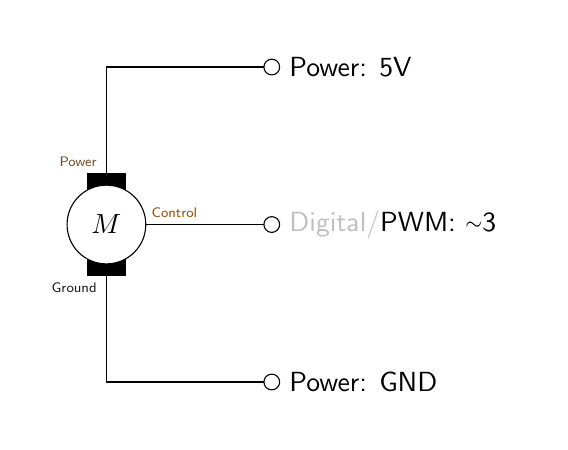
\begin{tikzpicture}[circuit ee IEC]

        % Background
        \draw[draw=none,fill=white] (1,0.5) rectangle ++(6.5,5);

        % Labels
        \node[anchor=west,font=\sffamily] at (4.2,5) {Power: 5V};
        \node[anchor=west,font=\sffamily] at (4.2,3) {\textcolor{gray!50}{Digital/}PWM: {\raise.17ex\hbox{$\scriptstyle\mathtt{\sim}$}}3};
        \node[anchor=west,font=\sffamily] at (4.2,1) {Power: GND};        

        % Motor
        \draw[draw=none,fill=black] (1.75,3.4) rectangle ++(0.5,0.25);
        \draw[draw=none,fill=black] (1.75,2.6) rectangle ++(0.5,-0.25);
        \draw[fill=white] (2,3) circle(5mm);
        \node at (2,3) {$M$};
        % Motor: Labels
        \node[anchor=east,font=\sffamily\tiny,text=black!40!brown] at (2,3.8) {Power};
        \node[anchor=west,font=\sffamily\tiny,text=black!40!orange] at (2.45,3.15) {Control};
        \node[anchor=east,font=\sffamily\tiny,text=black!90] at (2,2.2) {Ground};

        % Circuit
        \foreach \y/\len/\curve in {1/-2/1.4,3/-1.5/0,5/-2/-1.4} {
            \draw (4.1,\y) circle(1mm);
            \draw (4,\y) -- ++(\len,0) -- ++(0,\curve);
        }

    \end{tikzpicture}
\end{document}